%文档类型
\documentclass[a4paper]{article}

%引用包裹
\usepackage{bm}
\usepackage{cmap}
\usepackage{cite}
\usepackage{color}
\usepackage{float}
\usepackage{xeCJK}
\usepackage{amsthm}
\usepackage{amsmath}
\usepackage{amssymb}
\usepackage{booktabs}
\usepackage{setspace}
\usepackage{geometry}
\usepackage{hyperref}
\usepackage{enumerate}
\usepackage{indentfirst}
\usepackage[cache=false]{minted}

%页面格式
\geometry{margin=1in}

%字体设置
\setmainfont{Helvetica-Light}

%自定义宏
\newcommand{\norm}[1]{\left\lVert#1\right\rVert}

%正文部分
\begin{document}

%文章标题
\title{Magi Compiler Features}
\author{
	Zhijian Liu, F1403024, 5140309551\\
	\texttt{zhijianliu.cs@gmail.com}
}
\date{\today}

\maketitle

%正文开始
\section{Object Oriented Programming}
\subsection{Where are the Java Codes}
\noindent
\texttt{/src/Compiler/FrontEnd/ConcreteSyntaxTree/Listener/*}\\
\texttt{/src/Compiler/FrontEnd/AbstractSyntaxTree/Type/ClassType/*}\\
\texttt{/src/Compiler/Environment/ClassTable.java}
\subsection{An Example}
\inputminted[mathescape]{java}{code/object-oriented-programming/oop-2.mx}
\subsection{Advisory Test Case}
\noindent
\texttt{/report/bonus/data/object-oriented-programming/*}

\section{Single Static Assignment}
\subsection{Where are the Java Codes}
\noindent
\texttt{/src/Compiler/BackEnd/ControlFlowGraph/Instruction/PhiFunctionInstruction.java}\\
\texttt{/src/Compiler/BackEnd/ControlFlowGraph/SingleStaticAssignment/*}
\subsection{How to Print the SSA Form}
\begin{itemize}
\item
\texttt{make all \&\& cd bin/}
\item
\texttt{vim data.mx}\\
\texttt{\# input a Magi language code}
\item
\texttt{java -jar Compiler.jar -ssa < data.mx > assem.s}\\
\texttt{\# `-ast` to print the AST,`-ir` to print the IR after optimized}
\item
\texttt{spim -file assem.s}
\end{itemize}
\subsection{Advisory Test Case}
\noindent
\texttt{/report/bonus/data/single-static-assignment/*}
\subsection{Normalized Benchmark Result (compared with other students implemented SSA)}
\begin{figure}[!htp]
	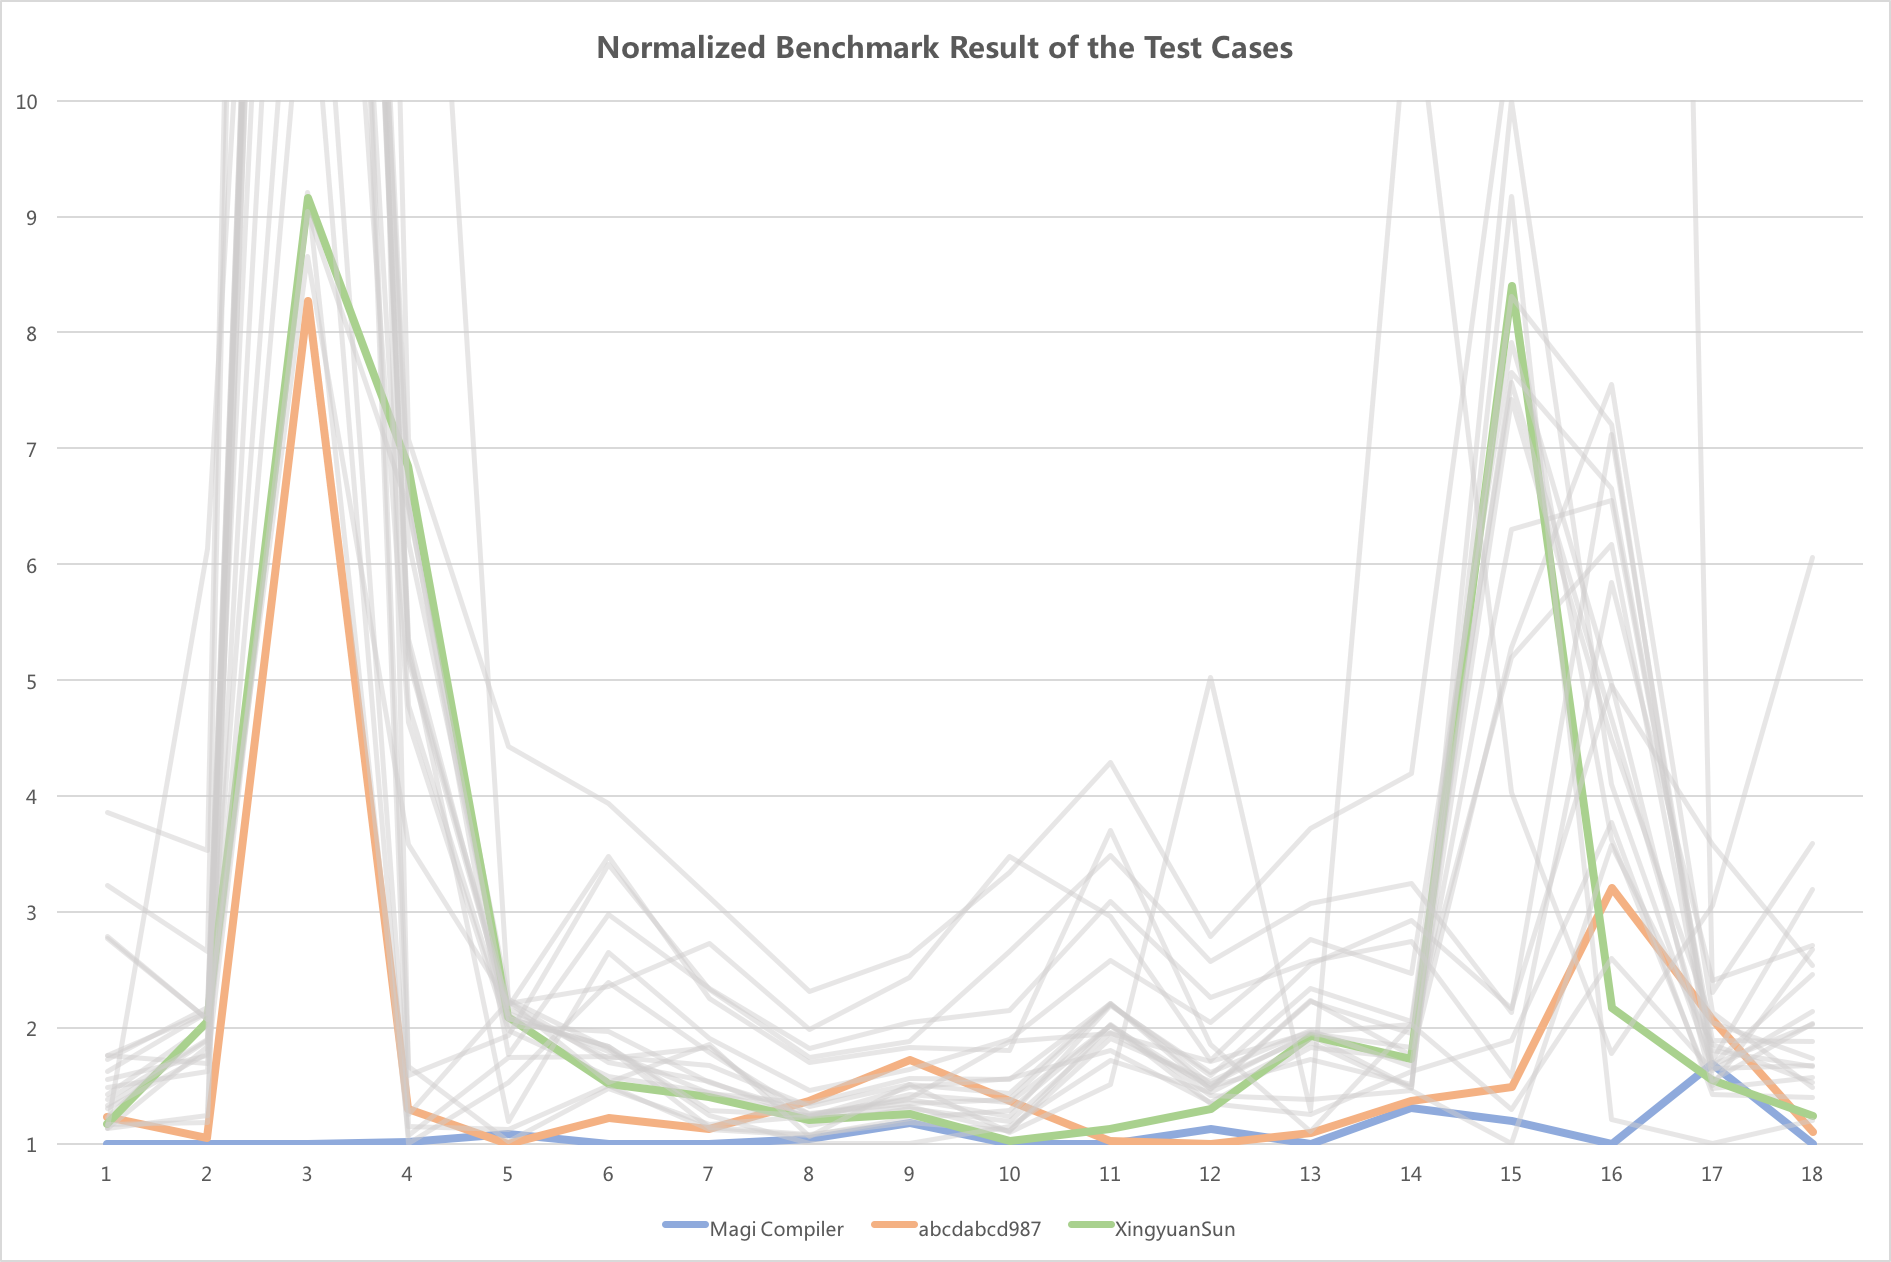
\includegraphics[width=\textwidth]{../presentation/image/benchmark/single-static-assignment}
\end{figure}

\section{Optimizations}
\subsection{Leaf Function Optimization}
\subsubsection{Where are the Java Codes}
\noindent
\texttt{/src/Compiler/BackEnd/Optimizer/LeafFunctionOptimizer.java}

\subsection{Control Flow Optimization}
\subsubsection{Where are the Java Codes}
\noindent
\texttt{/src/Compiler/BackEnd/Optimizer/ControlFlowOptimizer.java}

\subsection{Useless Code Elimination}
\subsubsection{Where are the Java Codes}
\noindent
\texttt{/src/Compiler/BackEnd/Optimizer/UselessCodeEliminator.java}

\subsection{Dominator-based Value Numbering Technique}
\subsubsection{Where are the Java Codes}
\noindent
\texttt{/src/Compiler/BackEnd/Optimizer/DbVNTOptimizer.java}

\subsection{Normalized Benchmark Result of the Optimizations}
\begin{figure}[!htp]
	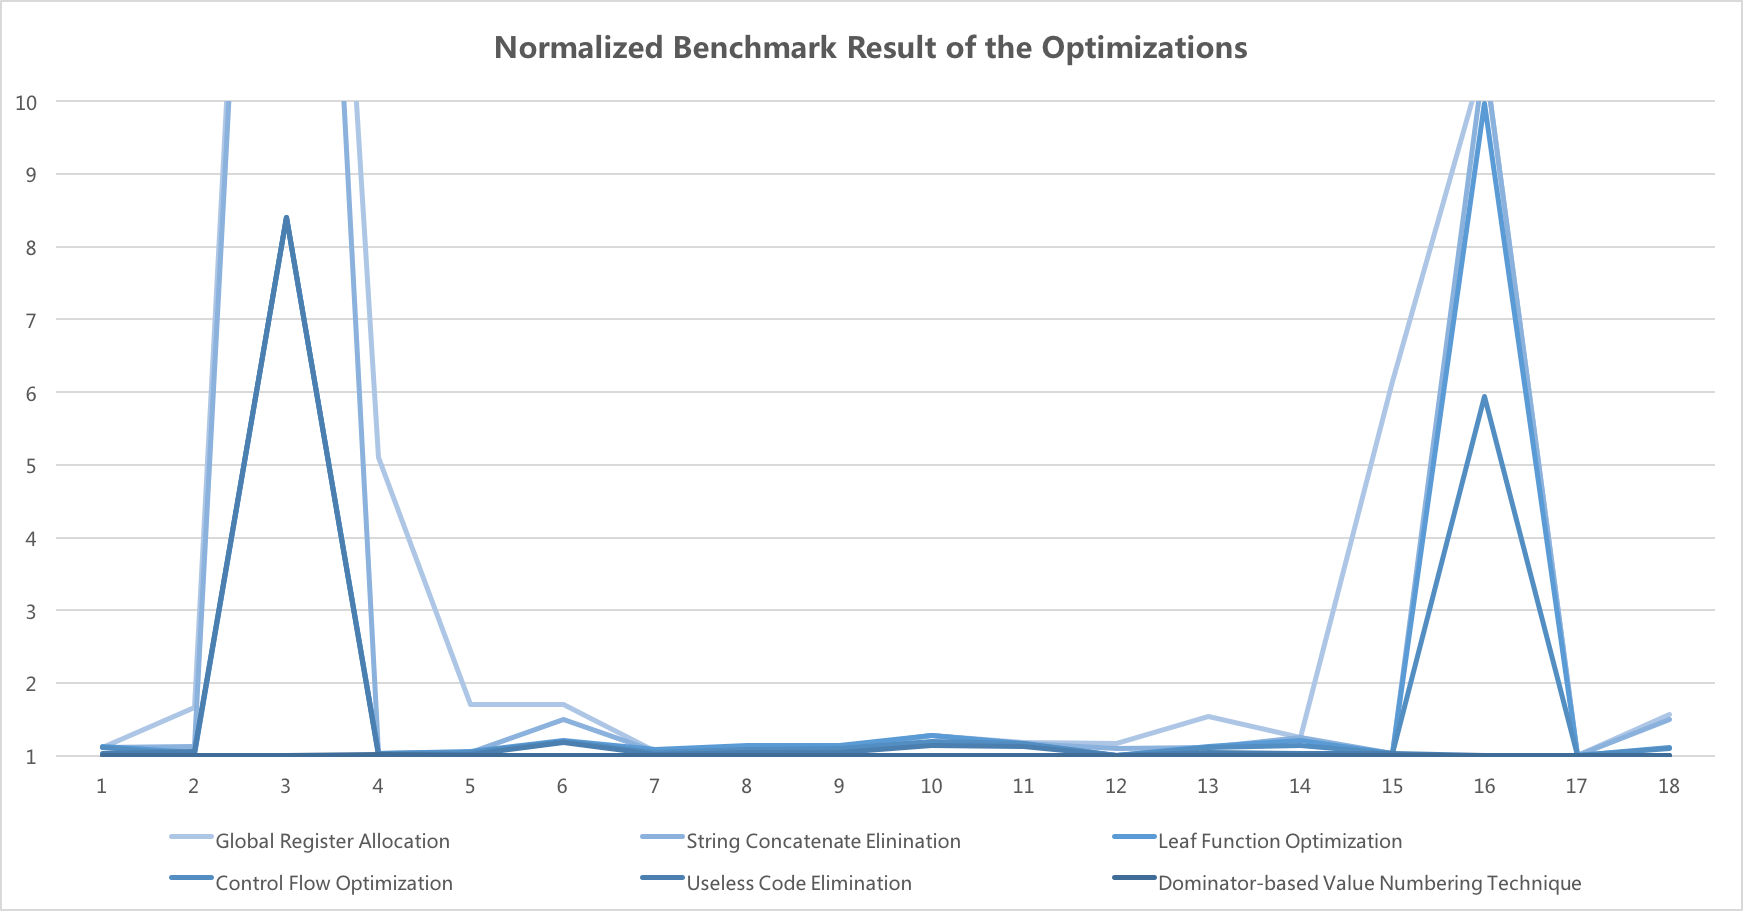
\includegraphics[width=\textwidth]{../presentation/image/benchmark/optimization}
\end{figure}

\section{Global Register Allocation}
\subsection{Where are the Code}
\noindent
\texttt{/src/Compiler/BackEnd/Allocator/*}

\subsection{Normalized Benchmark Result of the Register Allocation}
\begin{figure}[!htp]
	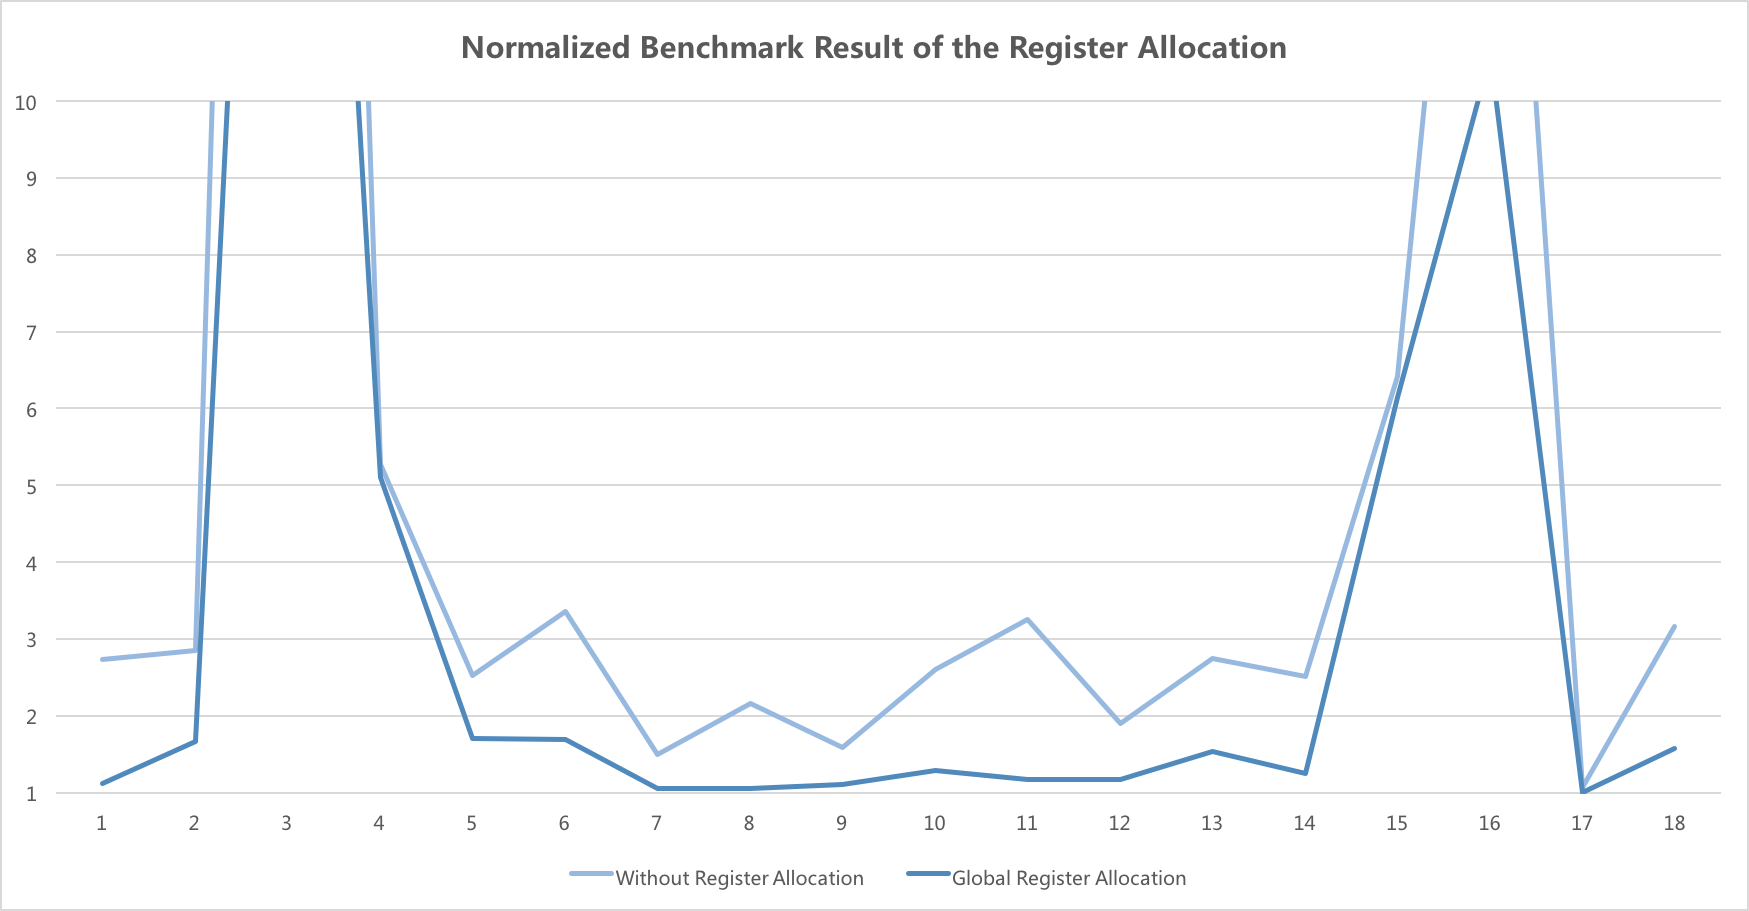
\includegraphics[width=\textwidth]{../presentation/image/benchmark/register-allocation}
\end{figure}

\section{Normalized Benchmark Result of the Test Case}
\begin{figure}[!htp]
	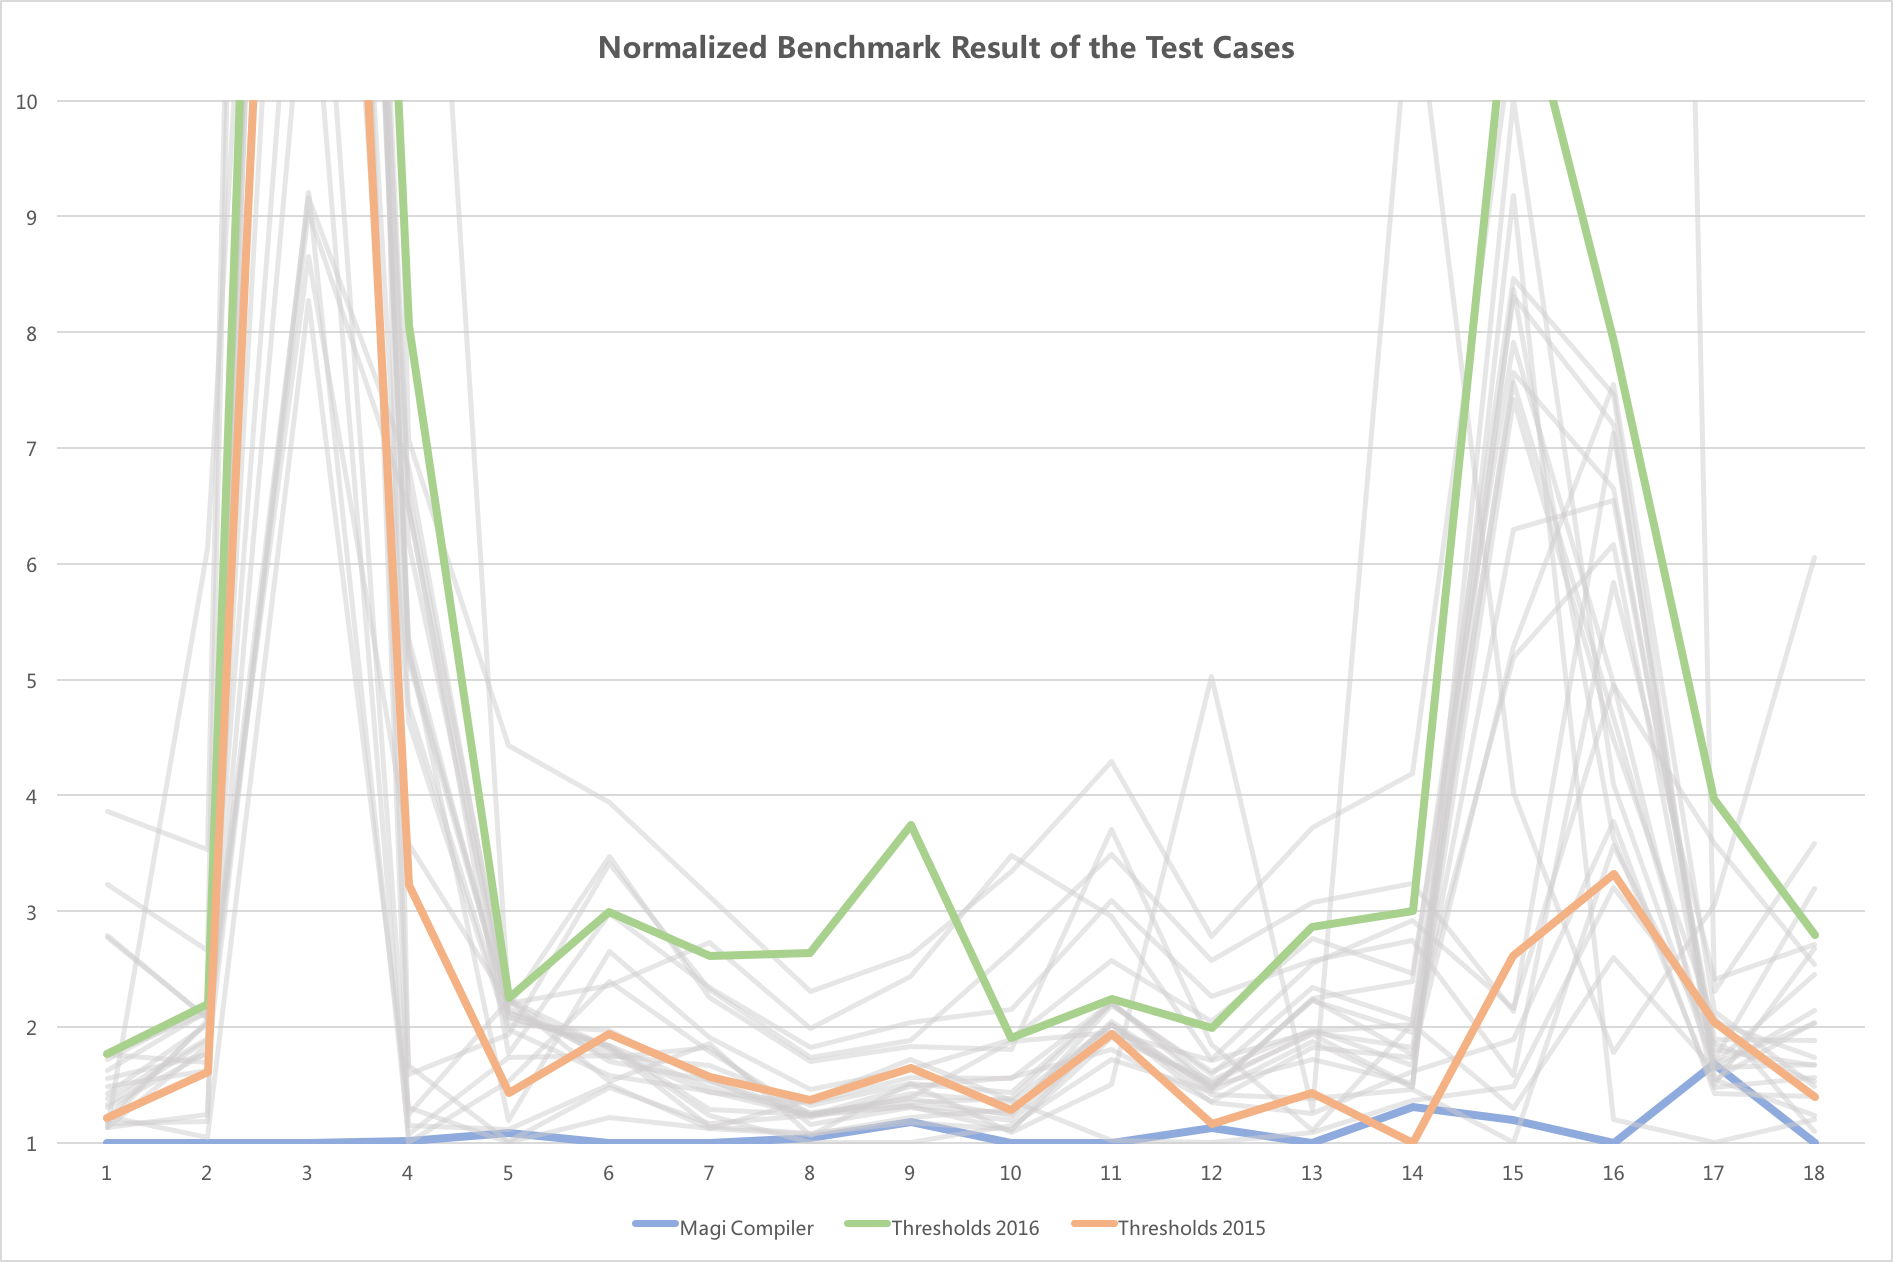
\includegraphics[width=\textwidth]{../presentation/image/benchmark/thresholds}
\end{figure}


\end{document}